\section{Structure du modèle}
\subsection{Modèle}
Dans le monde du reinforcement learning il existe plusieurs types de méthode d’apprentissage. L’une des méthodes d’apprentissage permettant d’obtenir les meilleurs résultats du fait de sa stabilité et la méthode de l’actor/critic.
Cette méthode consiste à créer deux modèles:

\begin{itemize}
    \item \textbf{Un actor:} 
    L’objectif de l'acteur est d’indiquer la politique à adopter (on parle en effet d’un acteur).
    Ainsi, c’est l’acteur qui choisit quelle action adopter en fonction de l’état dans lequel il se trouve.
    Il prend donc en entrée l’état de l’agent et il ressort en sortie l’action à adopter.
    
    \item \textbf{Un critic:} 
    Le critic comme son nom l’indique a pour but de critiquer l’action ou l’état du robot.
    En effet, cela dépend de la méthode employé.
    Il prend en entrée l’état de l’agent et ressort en sortie la valeur de l’état dans lequel se trouve l’agent.
\end{itemize}

\begin{figure}[H]
    \centering
    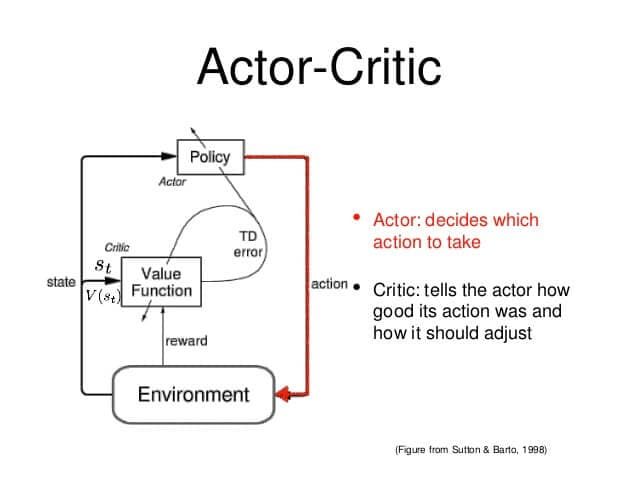
\includegraphics[width=0.5\textwidth]{./image_RL/image23.png}
    \caption{Actor-Critic, \textit{source : David Silver RL}}
\end{figure}

Nous avons donc utilisé la même structure que celle décrite dans l’article suivant [4].
